\section{Post Service}{Jose I. Retamal }
Jose I. Retamal
\vskip 0.1in
\indent
\indent
Post Service manage posts, there are posts for cities and places. The service is composed of two paint parts: The main service and the database(Fugure \ref{post:mainuml}).
 
The main service connects to the client and provides the main endpoints for creating view and update posts. It connects to the Mongo database and checks requests on the authentication service. 


\begin{figure}[H]
	\begin{center}
		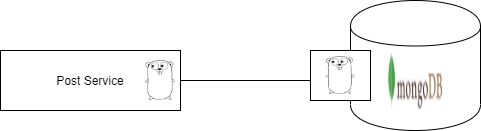
\includegraphics[width=120mm,scale=1]{img/post/post-main-uml.png}
		\caption{Post Service- UML.}
		\label{post:mainuml}
	\end{center}
	
\end{figure}

\subsection{Request Sequence}

\begin{itemize}
	\item Create Post 
	
	When a user creates a post, the request contains the post data and the authentication token. The token is check in the authentication service, and then the post is stored in the database.
\end{itemize}

\subsection{The database}

Post are grouped by place and cities using the Neo4j unique id for each city and place. The database is composed of two tables, one for cities and another for places(Figure \ref{post:dbentity}).
All data is stored in one collection. The data is indexed by the unique id (index id) therefore, the performance is not affected by the amount of data stored.

\begin{figure}[H]
	\begin{center}
		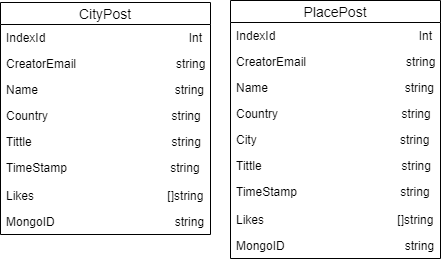
\includegraphics[width=90mm,scale=1]{img/post/post-db-entity.png}
		\caption{Post Service- Database Entity Diagram.}
		\label{post:dbentity}
	\end{center}
\end{figure}

\section{The rest API}
 \indent
 \indent
The rest API provides access to all services, combines the data, and create a single JSON response. 

The API has been documented online using PostMan : \url{https://documenter.getpostman.com/view/11354288/SzmfYHa4?version=latest} 

The requests that are implemented are:
\begin{itemize}
	

\item Create User
\item Log In
\item  Log out 
\item  Update User
\item  Create City
\item  Get City
\item  Update City
\item  Create Place
\item  Get Place
\item  Get All City Places

\end{itemize}
